\documentclass[12pt,titlepage,french]{article}
\usepackage{babel}
\usepackage{graphicx}
\usepackage[margin=2.5cm]{geometry}

\usepackage[hidelinks]{hyperref}
\usepackage{tabularx}
\usepackage{float}
\usepackage[utf8]{inputenc}
\usepackage[T1]{fontenc}
\pagestyle{plain}

\usepackage{booktabs,makecell,tabu}
\usepackage{comment}
\renewcommand\theadfont{\bfseries}

\linespread{1.5}

\newcounter{firstbib}

\begin{document}
%\renewcommand{\thesection}{\arabic{section}} % utilisé pour spécifier la numérotation des sections

\begin{titlepage}
\newcommand{\HRule}{\rule{\linewidth}{0.5mm}}
\center

  
\includegraphics[width=0.45\textwidth]{../../ressources/img_logos/logo_polytech.png}\\[1cm]

  
\includegraphics[width=0.45\textwidth]{../../ressources/img_logos/logo_taglabs.png}


\HRule \\[0.4cm]
{ \huge \bfseries Rapport itération 6\\[0.15cm] }
Classification colorimétrique de nuages de points 3D\\
Version 1.0\\
Le \today \\
\HRule \\[1.5cm]
Ronan Collier,
Mathieu Letrone,
Tri-Thien Truong
\\[1cm]
\end{titlepage}

\tableofcontents % table des matières
\newpage
\listoffigures  % table des figures
\newpage

\section{Rappel des objectifs de l'itération}
Cette itération étant la dernière du projet, nous devions finaliser les fonctionnalités et corriger les derniers bugs relevés via le feedback. Il nous fallait aussi nous concentrer sur la réalisation de différents rapports, notamment le rapport de description du système beta et le rapport de recette.

Les tâches que nous nous sommes fixées sont les suivantes :

\begin{itemize}
    \item Désactivation des filtrages selon le nuage sélectionné
    \item Redéfinir les bornes RGB
    \item Implémentation du filtrage scalaire
    \item Réaliser les tâches du feedback (points externes/internes, indications, icônes)
    \item Finir algo k-means/autre algorithme
    \item Terminer algorithme sélection de points
    \item Faire le lien entre tone mapping et filtrage
\end{itemize}


\section{Production / réalisation durant l'itération}

Nous développerons ici chaque objectif que nous nous sommes fixé pour cette itération.


\subsection{Désactivation des filtrages selon le nuage}

Lors du test de notre plugin par le client et le créateur de CloudCompare, M. Daniel Girardeau-Montaut, un problème a été remonté notamment lorsque l'on utilisait un type de filtrage, pour un nuage de points qui ne le concernait pas. Par exemple, il était possible jusqu'au début d'itération de pouvoir appliquer le filtrage RGB pour un nuage de points en valeurs scalaires. Ce problème a été corrigé en désactivant les filtrages selon le nuage sélectionné. \newline

Pour faire cela, nous avons deux booléens : un pour vérifier si le/les nuages sélectionnés sont en couleurs, et l'autre booléen pour les valeurs scalaires. \newline

Il est possible ensuite de vérifier via la méthode "hasColors" et "hasDisplayedScalarField" d'un objet "ccHObject" nos conditions. Il nous suffit ensuite d'activer ou non les boutons permettant aux filtrages, grâce à nos deux booléens. \newline

Nous avons aussi défini que si un nuage en couleurs et un nuage en valeurs scalaires sont sélectionnés, nous n'activons aucun bouton.

\begin{figure}[H]
 \caption{\label{} Exemple d'un nuage en couleurs}
 \begin{center}
 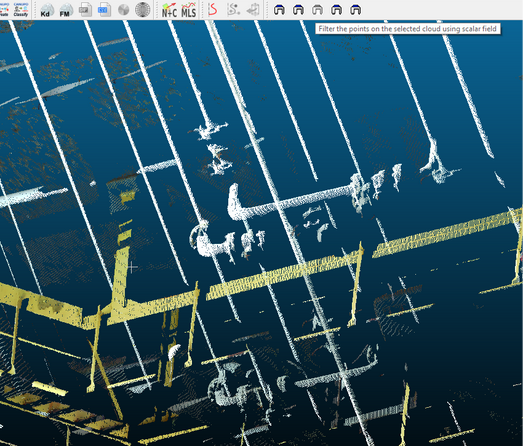
\includegraphics[width=1\textwidth]{./img/color_cloud.PNG}
  \end{center}
\end{figure}

\begin{figure}[H]
 \caption{\label{} Exemple d'un nuage en gris}
 \begin{center}
 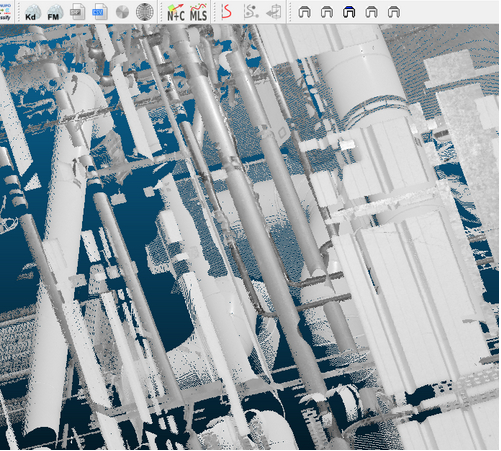
\includegraphics[width=1\textwidth]{./img/grey_cloud.PNG}
  \end{center}
\end{figure}

\subsection{Redéfinir les bornes RGB}

Lors de l'itération précédente, nous avons voulu réfléchir à un moyen pour détecter automatiquement les bornes minimum et maximum du filtrage RGB. En effet, lorsque l'utilisateur choisissait un point avec des valeurs élevées en tant que premier point, et des valeurs faibles pour le second, notre filtrage ne pouvait pas bien fonctionner. \newline

Nous avons essayé d'utiliser l'espace colorimétrique HSV pour déterminer quel point était plus sombre que l'autre, notamment avec la Saturation et la Valeur, mais nous nous sommes rendu compte que cela était trop complexe et pas forcément viable. \newline

La dernière solution qui a été retenue, et la plus simple à implémenter, est le fait de déterminer la valeur minimum et maximum pour chaque composante RGB entre les deux points. On aurait alors deux potentielles nouvelles couleurs, selon les valeurs des points sélectionnés.

\begin{figure}[H]
 \caption{\label{} Exemple filtrage RGB}
 \begin{center}
 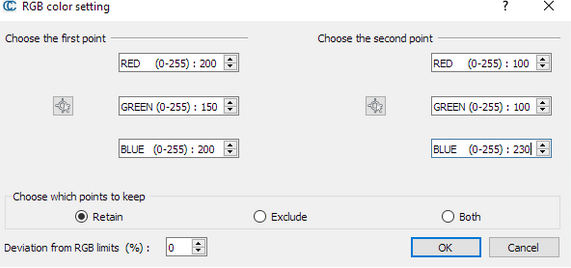
\includegraphics[width=1\textwidth]{./img/rgb_ui.PNG}
  \end{center}
\end{figure}

\begin{figure}[H]
 \caption{\label{} Résultat des bornes du filtrage RGB}
 \begin{center}
 
\includegraphics[width=1\textwidth]{./img/rgb_res.PNG}
  \end{center}
\end{figure}

Dans cet exemple, nous pouvons constater que dans le premier point sélectionné, les valeurs des composantes Rouge et Vert sont supérieures que dans le deuxième point. \newline

Dans le résultat, nous avons utilisé les valeurs Rouge et Vert du deuxième point, en tant que borne minimum. La nouvelle couleur qui servira de borne inférieure est donc "100/100/200" et supérieure "200/150/230".

\subsection{Implémentation du filtrage scalaire}
% TODO

\subsection{Tâches du feedback : points externes/internes}

Nous avons ajouté une fonctionnalité qui est maintenant disponible pour tous les types de filtrages, qui est le choix des points à garder. En effet, précédemment, nous gardions uniquement les points qui respecte les bornes définies par l'utilisateur, donc nous gardions uniquement les points similaires au choix de l'utilisateur. Maintenant, il est possible de choisir si l'utilisateur veut garder ces points, ou les points qui sont hors des bornes. Cela permet à l'utilisateur de supprimer certains points, en utilisant nos filtrages. \newline

\begin{figure}[H]
 \caption{\label{} Choix des points à garder}
 \begin{center}
 
\includegraphics[width=1\textwidth]{./img/choix.PNG}
  \end{center}
\end{figure}

Ici, nous pouvons voir que nous avons trois choix.  Le choix de l'option "Retain" permet à l'utilisateur de créer un sous-scan où les points affichés seront les points qui sont à l'intérieurs des bornes. Inversement, l'option "Exclude" va permettre de créer un sous-scan avec les points qui seront hors de l'intervalle choisi. Enfin, la dernière option "Both" va permettre de réaliser les deux options. Nous aurons donc à la fin, deux sous-scans où la somme va permettre de retrouver le scan original.

\begin{figure}[H]
 \caption{\label{} Résultat du scan pour les points du choix "Retain"}
 \begin{center}
 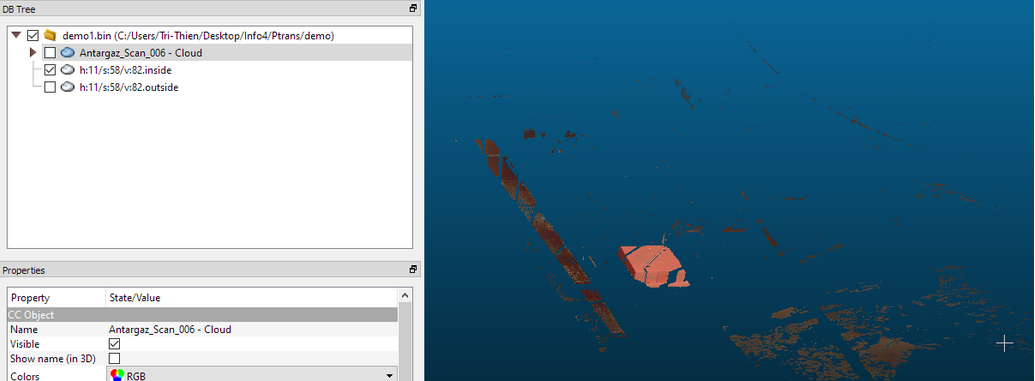
\includegraphics[width=1\textwidth]{./img/choix_ex_1.PNG}
  \end{center}
\end{figure}

\begin{figure}[H]
 \caption{\label{}  Résultat du scan pour les points du choix "Exclude"}
 \begin{center}
 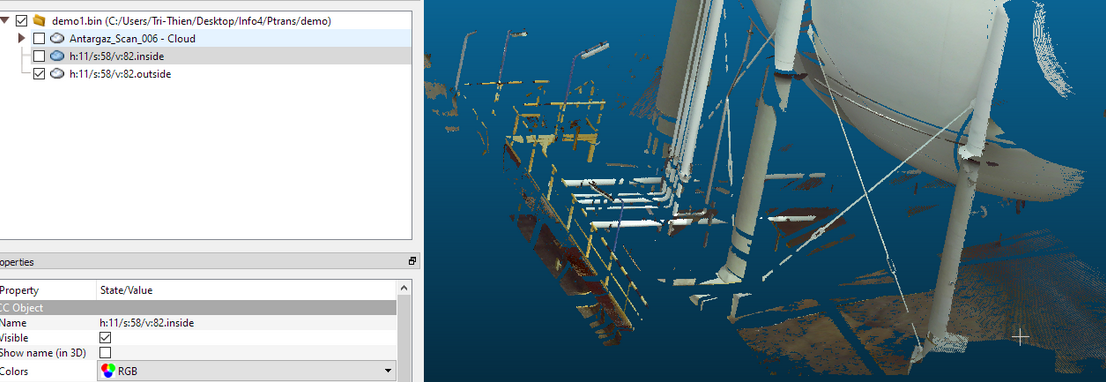
\includegraphics[width=1\textwidth]{./img/choix_ex_2.PNG}
  \end{center}
\end{figure}

\subsection{Tâches du feedback : icônes}
% TODO

\subsection{Algo K-means}
% TODO

\subsection{Fin de l'implémentation de l'algorithme de sélection de points}
% TODO

\subsection{Lien Tone mapping et filtrages}
Après avoir développé le Tone mapping, il nous fallait faire des tests avec nos algorithmes de filtrages, et ainsi voir les résultats obtenus.

\begin{figure}[H]
 \caption{\label{}  Exemple d'application du tone mapping : scan original}
 \begin{center}
 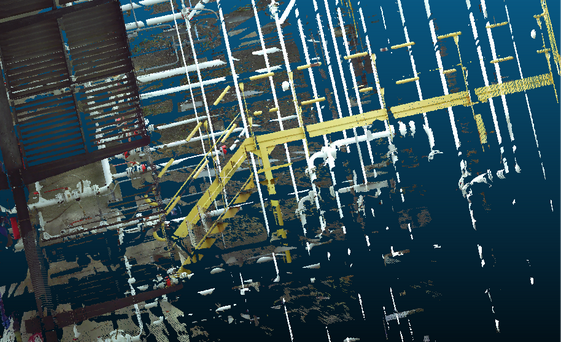
\includegraphics[width=0.8\textwidth]{./img/tm_example_1.PNG}
  \end{center}
\end{figure}

\begin{figure}[H]
 \caption{\label{}  Exemple d'application du tone mapping : scan avec tone mapping}
 \begin{center}
 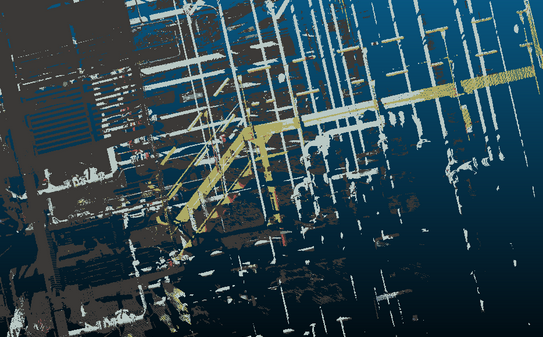
\includegraphics[width=0.8\textwidth]{./img/tm_example_2.PNG}
  \end{center}
\end{figure}

\begin{figure}[H]
 \caption{\label{}  Exemple d'application du tone mapping : scan filtré}
 \begin{center}
 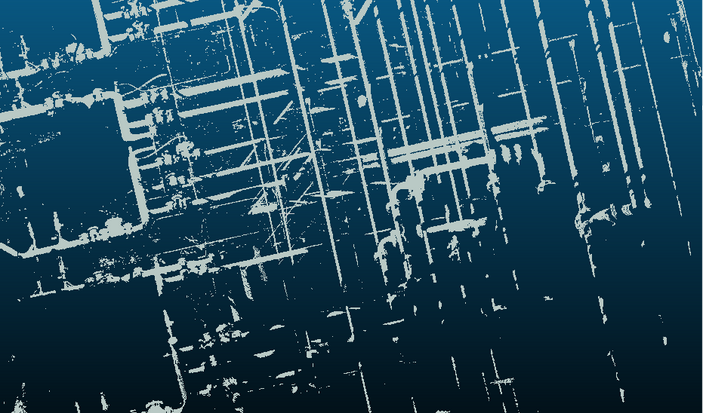
\includegraphics[width=0.8\textwidth]{./img/tm_example_3.PNG}
  \end{center}
\end{figure}

Nous avons appliqué sur le scan original, du tone mapping avec 8 couleurs. Nous pouvons voir qu'une partie des points jaunâtres à été considéré comme du blanc, car les points étaient très claires. Après filtrage, nous avons voulu gardé que les points blancs, afin de mettre en valeur les tuyaux blancs. Nous avons des bons résultats, puisque nous avons même les points gris des tuyaux qui sont cachés, mais nous avons aussi du résidu, comme les points blancs de l'escalier jaunâtre.

\section{Risques éliminés durant l'itération}

Durant cette dernière itération, nous avons pu terminer de nombreux bugs qui pouvait faire planter l'application. Malheureusement, nous n'avons pas pu obtenir des résultats satisfaisants pour l'algorithme de sélection de points, que nous avons donc arrêté par manque de temps.

\section{Feedback}


\section{Commentaires sur l'itération}

Cette section va présenter nos ressentis sur notre itération. Cela peut correspondre à la façon dont nous avons pu gérer la charge de travail que nous avions prévu en début d'itération, des potentiels imprévus, points positifs/négatifs, et autres.

\subsection{Commentaires sur l'itération de façon générale}

Cette itération s'est plutôt bien déroulé de façon générale. Nous avons eu du temps pour travailler sur le projet. Nous avons quand même accordé beaucoup de temps sur la mise au propre du code et des différents rapports, afin de préparer le rendu final du projet transversal.

\subsection{Commentaires sur les méthodes de travail/changements de méthode}

Nos méthodes de travail ont été les mêmes que pour les autres itérations.

\end{document}
